\section{Methodology} \label{sec:methodology}

To investigate the effect of explainable generative \ac{AI} on users' problem-solving process and their metacognitions a grounded-theory approach based on \textcite{Gioia2013} was chosen. The grounded-theory approach is well-suited for exploratory research, as it allows for the development of theories from empirical data. The two-step analysis process allows to retain a connection between the data and the theoretical results \parencite{Gioia2021}. This is particularly important in the context of human-\ac{AI} interaction, as the field is still relatively new and theories are still being developed. The following sections will present the design and execution of the study, as well as the procedure for data analysis inspired by \textcite{Jussupow2021}.

\subsection{Research Design} \label{ssec:research_design}

The study is a mixed-method study where the participants were tasked with solving maths problems with the help of a chatbot, that was tuned to assist the users without solving the problems for them. Qualitative data about the problem-solving approach was collected as think-aloud protocols, while additional quantitative data about the perception of the chatbot was recorded using questionnaires. To investigate the effects of explanations, participants were split into two separate groups, that provided different chatbots: Group (E) was using a chatbot, that provided an explanation for its outputs, group (B) did not receive an explanation. Both groups were served tasks from the same pool and answered the same questionnaires after completing the tasks. The goal was to perform a between-subjects comparison of the two groups to identify differences in problem-solving strategies and metacognitive processes.

\subsubsection{Tasks} \label{sssec:tasks}

The problems given to the participants needed to be of sufficient complexity to require assistance from the chatbot, while still being solvable by a wide range of potential participants. Ideally the problems should offer multiple solution strategies, to allow for a variety of approaches. The problems were selected form an existing dataset inspired by \textcite{Wang2024}. While the MathVista dataset \parencite{MathVista2024} was designed for evaluating \ac{AI} systems, it can be reused for this study, since the problems are posed in natural language and often require combining visual and textual information to solve them. The selection was performed to ensure that the problems were solvable by \ac{STEM}-students, taking into account the clarity and difficulty of the problems. The final selection consisted of 15 problems from the domain of geometry.

Participants were given sets of three random problems selected, with the constraint that only “medium” and “difficult” problems were included during the study. The problems were presented digitally in a custom web application. The participant were shown the task image, text, and answer options at once. The tool recorded participants responses and time taken to solve the tasks. In case a participant was unable to solve a problem, it was replaced by a new problem of the same difficulty.

\subsubsection{Chatbot Design} \label{sssec:chatbot_design}

The chatbot used for the study needed to be created specifically for the purpose of the study, as no existing chatbot fulfilled the requirements of the study. The design was driven by several requirements and constraints, derived from the research questions and practical considerations. The main consideration was to ensure that the chatbot would assist the participants, without solving the problems for them. Additionally, the chatbot should support image inputs, as the problems included visual information. Lastly, that chatbot should be able to provide a \ac{CoT} explanations, to allow for comparison between users with and without explanations.

In addition to the research-related requirements described above, practical considerations also influenced the design and implementation of the chatbot. The chatbot needed to be either runnable on a laptop or accessible via a free API, to keep the cost of the study low. Additionally, the implementation of the chatbot should be build using existing software as much as possible. Due to a lack of free API options that sufficed the research requirements, the chatbot was implemented locally using LM Studio \parencite{ElementLabs2025}, which allowed to experiment with different models and configurations before the study. It also allowed to easily experiment with additional system prompts, that could be used to tailor the responses of the model to the specific use case.

The available models were filtered automatically to only include models that were runnable on a M4 MacBook Pro (12cpu, 24 GB RAM) according to the program. After curating the list of available models and eliminating identical models of different sizes, the following options remained:

\begin{itemize}
    \item Qwen 3 (30B A3B) lacks vision capabilities, but has the unique ability to turn \ac{CoT} explanations on and off using the \texttt{/nothink} command in prompts \parencite{Qwen2025}.

    \item Gemma 3 (27B) offers vision capabilities and is the largest model, that can reliably be used on the device available. It lacks explicit \ac{CoT} explanation capabilities \parencite{GemmaTeam2025}.

    \item Mistral Small 3.2 is the newest of the three architectures and has vision capabilities. Like Gemma 3 it lacks \ac{CoT} explanations \parencite{Mistral2025}.
\end{itemize}

Initial experiments performed by the researcher before the study yielded, that vision capabilities would likely be of high importance. This meant Qwen 3 would need to be equipped with visual capabilities. Additionally, Qwen struggled with following the system prompts, forbidding to reveal the solution to the user, especially when \ac{CoT} explanations where enabled. It was therefore removed from the shortlist.

The remaining two models were tested using identical 2 identical system prompts. Both prompts instructed the model to act as helpful assistant, that would not solve the maths problems for the user, but instead provide guidance and hints. The difference between the prompts was that one prompt instructed the model to provide a \ac{CoT} for each response wrapped in a \texttt{<think>} tag. Both versions of the prompt can be found in the appendix. The results of the tests showed, that Mistral Small 3.2 was more reliable in following the instructions, while Gemma 3 often revealed the solution to the user, despite the system prompt. Mistral Small 3.2 was therefore chosen as the model for the chatbot.

\subsubsection{Experiment Procedure} \label{sssec:experiment_procedure}

At the beginning of the experiment, the participants were given a short introduction to the study and the tools they would be using. This introduction included a demonstration of the chatbot in form of an example task solved by the researcher with help of the chatbot\footnote{The demonstration followed a script, that included the demonstration of the vision capabilities of the chatbot and specifically pointed out the explanations to participants of group (E)}. After explaining the concept of think-aloud protocols, they were given a practice task and feedback afterwards. During the study the participants were asked to solve three randomly selected tasks after one another. An example task is shown in figure \ref{fig:task_viewer}. They were given the chatbot (opened in a separate window from the tasks), a scientific calculator, and pen and paper for making notes. They were allowed to freely use all assistance they were offered at their discretion and afforded as much time as they wanted to solve tasks. Once users completed the tasks, they were given a set of questionnaires to fill out.

\begin{figure}[ht]
    \centering
    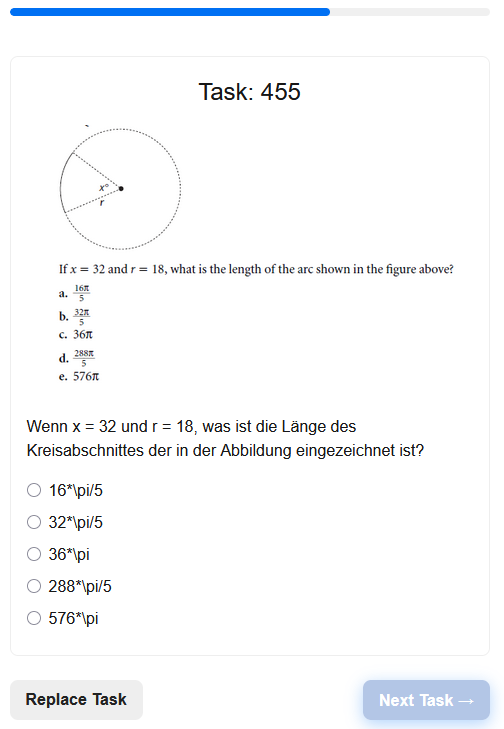
\includegraphics[width=0.4\textwidth]{images/fig-task_viewer.png}
    \caption{Task viewer used in the experiment to present the tasks to the participants.}
    \label{fig:task_viewer}
\end{figure}

During the experiment qualitative and quantitative data was collected in several ways. Qualitative data was primarily collected by conducting experiments using the think-aloud method \parencite{VanSomeren1994}. Additionally, the conversation of users with a chatbot were recorded, to be combined with the transcripts of the think aloud protocols. A cover story was provided to the users for the experiment, telling them the goal of the study was the evaluation and comparison of the different chatbot versions \parencite{VanSomeren1994, Jussupow2021}. Lastly some participants proactively provided additional feedback after completing the experiment, which was recorded with notes by the researchers. The data was transcribed using OpenAI Whisper \parencite{Radford2022} using the “medium” sized model and specifying German as language. Afterwards the transcripts were validated against the original audio recordings and combined with the applicable chat histories to a single transcript per task.

Quantitative data was gathered using a number of post-experiment questionnaires to gather data about user's acceptance, self-efficacy, and mental load during the tasks. The questionnaires used were \ac{TAM} \parencite{Davis1989}, \ac{CSE} \parencite{Compeau1995}, and \acs{NASA}-\ac{TLX} \parencite{Hart1988}. As the study was performed in German translations for the questions and responses were required. Research showed, the \acs{NASA}-\ac{TLX} questionnaire \parencite{Flaegel2019} and \ac{TAM} \parencite{Jockisch2010} were available translated and validated, but both versions were adopted for specific studies, which made them insufficient for this study. Therefore, the questionnaires were manually translated. The translations can be found in the Appendix.

\subsubsection{Participants} \label{sssec:participants}

Participants were selected from university students, colleagues, friends, and acquaintances. The primary requirement for participants was a background in \ac{STEM}, either through their studies or profession. This was to ensure that participants had sufficient prior maths knowledge to solve the problems. The participants were split into two groups pseudo randomly in order of their registration, alternating between the two groups.

\subsection{Data Analysis} \label{ssec:data_analysis}

The data analysis was divided into qualitative and quantitative analysis, which were performed separately and then combined during the interpretation of the results. The procedure for both will be described in the following sections.

\subsubsection{Qualitative Analysis} \label{sssec:qualitative_analysis}

The qualitative data was analysed using a grounded-theory approach and focused on retaining the data-to-theory connection \parencite{Gioia2021}. Aligned with the structure proposed by grounded-theory research, the analysis was performed in two cycles following the example of \textcite{Jussupow2021} and general methodology for coding outlined by \textcite{Saldana2015}. The first cycle focused on getting an overview of the data and extracting relevant information from the transcripts. The second cycle coding iterations served to group and organize the codes from the first cycle and connect them to existing theory. The following coding methods cycles were performed (using the terminology of \textcite{Saldana2015}):

\begin{enumerate}
    \item \textbf{First Cycle Coding:}
    \begin{enumerate}
        \item \textbf{Descriptive Coding}: The first cycle started with descriptive coding, to get an initial overview of the data.
        \item \textbf{Process Coding}: The second step was process coding, to extract relevant process steps and elements from the transcripts.
    \end{enumerate}
    \item \textbf{Second Cycle Coding:}
    \begin{enumerate}
        \item \textbf{Axial Coding}: The codes from the first cycle were then grouped and organized using axial coding.
        \item \textbf{Theoretical Coding}: Finally, theoretical coding was used to develop a theory or process model from the previously grouped codes.
    \end{enumerate}
\end{enumerate}

\subsubsection{Quantitative Analysis} \label{sssec:quantitative_analysis}

Quantitative data was collected and evaluated to complement the qualitative data. The primary goal of the quantitative data analysis was to determine differences between the two chatbot versions with regard to user acceptance and mental load. The questionnaires were evaluated according to the instructions provided in the original publications. The results were then compared between the two groups to identify any significant differences between the different chatbot versions.

In accordance with the original publications the scores for TAM and CSE were calculated as the mean of the respective questionnaire items, where TAM was split into the two dimensions \textit{perceived usefulness} and \textit{perceived ease of use} \parencite{Davis1989,Compeau1995}. The \acs{NASA}-\ac{TLX} questionnaire was evaluated on four of the six subscales. The subscales for \textit{physical load} and \textit{temporal demand} were excluded from the evaluation, since there was no significant physical effort required and no time limit set for the tasks. The scale for \textit{performance} needed to be inverted, since the question is posed with an inverted scale compared to all other questions in the \acs{NASA}-\ac{TLX} questionnaire. In accordance with \textcite{Hart2006} the \ac{TLX} constructs were evaluated using the “raw TLX” (sometimes called “RTLX”) to reduce the data collection and evaluation effort. This results in an overall investigation of seven constructs across the three questionnaires:

\begin{itemize}
    \item Perceived Usefulness (\ac{TAM})
    \item Perceived Ease of Use (\ac{TAM})
    \item Self-Efficacy (\ac{CSE})
    \item Mental Demand (\acs{NASA}-\ac{TLX})
    \item Performance (\acs{NASA}-\ac{TLX})
    \item Effort (\acs{NASA}-\ac{TLX})
    \item Frustration (\acs{NASA}-\ac{TLX})
\end{itemize}

To determine if there were significant differences between the two groups, a Mann-Whitney U test was performed for each of the seven constructs. The Mann-Whitney U test was chosen, as it does not assume normal distribution of the data and is suitable for small sample sizes. Due to the small sample size the goal of the analysis was to identify potential trends in the data, rather than to draw definitive conclusions. Therefore, a significance level of $\alpha = 0.1$ was chosen for the analysis.

The evaluation of the questionnaires was performed using Python with the libraries Pandas and SciPy. Technical details about the evaluation the questionnaires can be found in the code repository accompanying this thesis \parencite{Goepfert2025}.
